\documentclass[]{article}

%opening
\title{no title}
\date{\today}
\usepackage{amssymb}
\usepackage{amsmath}
\usepackage{tikz-cd}
\usepackage{quiver}
\usepackage{graphicx}

\newtheorem{theorem}{Theorem}
\newtheorem{definition}{Definition}
\newtheorem{lemma}{Lemma}

\newcommand{\C}{\mathbb{C}}
\newcommand{\Hom}{\text{Hom}}
\newcommand{\Hol}{\text{Hol}}
\newcommand{\Ann}{\text{Ann}}
\newcommand{\OO}{\mathcal{O}}
\newcommand{\LL}{\mathcal{L}}
\newcommand{\MM}{\mathcal{M}}
\newcommand{\End}{\text{End }}
\newcommand{\coker}{\text{coker}~}
\newcommand{\dbar}{\overline{\partial}}
\newcommand{\cA}{\mathcal{A}}
\newcommand{\cG}{\mathcal{G}}
\newcommand{\cP}{\mathcal{P}}
\newcommand{\Tr}{\text{Tr }}
\newcommand{\HH}{\mathbb{H}}
\newcommand{\XX}{\mathfrak{X}}
\newcommand{\QQ}{\mathfrak{Q}}
\newcommand{\sslash}{\mathbin{/\mkern-4mu/}}

\begin{document}
	In sections 2, 3 and 4, we have described the moduli space $\MM$ of flat $SU(2)$ connections on a compact Riemann surface $\Sigma$, and the corresponding spaces $P$ and $\cP$ of representations with weighted frames on $\Sigma$ and framed parabolic sheaves on $\tilde{\Sigma}$, a singular curve corresponding to $\Sigma$ via degeneration. Now in this section we will describe how this degeneration of $\Sigma$ to $\tilde{\Sigma}$ induces a degeneration of $\MM$ to $\cP$. This degeneration of moduli spaces is due to the work of Biswas and Hurtubise (cite). Furthermore, we will describe a recent result of Harada and Kaveh (cite) which tells us that under certain hypotheses, the integrable system on $\MM$ described in section 3 yields an integrable system on $\cP$.
\subsection{Degeneration of the Curves}
	The relationship between the moduli spaces $\MM$ and $\cP$ is given by degenerating the Riemann surface $\Sigma$ to a nodal curve by smoothly shrinking the boundary curves of the trinion decomposition. First we describe a local model for this shrinking process.
	
	\begin{figure}[h]
		\centering
		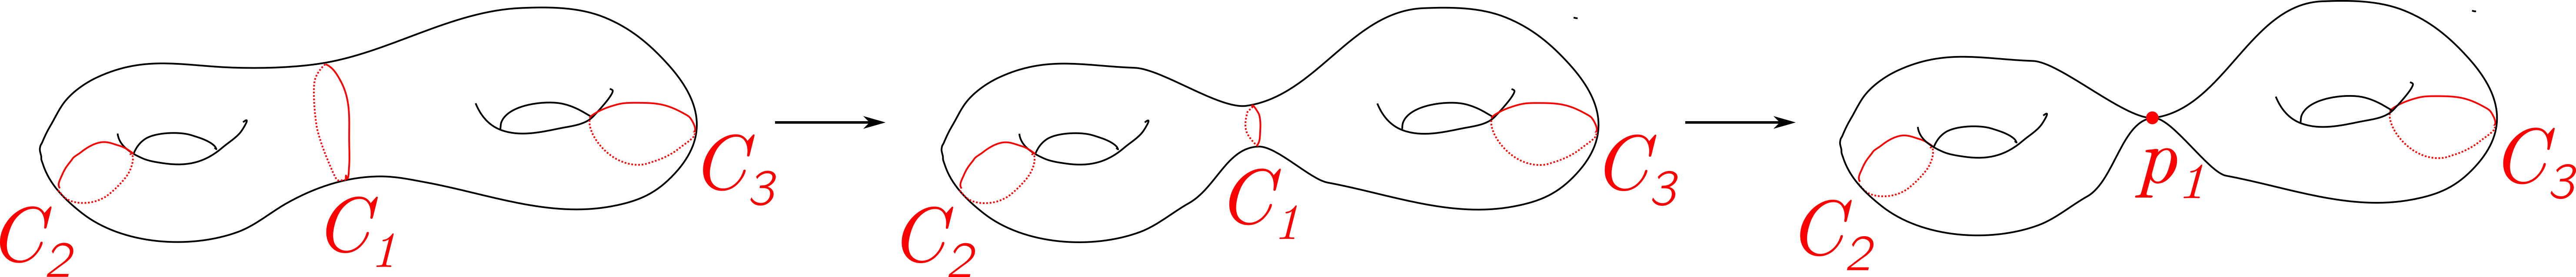
\includegraphics[width=0.6\linewidth]{degen1pt}
		\caption{Smoothly shrinking one boundary curve to a point.}
		\label{fig:degen}
	\end{figure}
	
	Let $\Sigma$ be a compact connected Riemann surface of genus $g$ as before. Let $\Sigma_0$ denote the nodal curve obtained by trinion decomposition from $\Sigma$, replacing each boundary circle of the trinions with a single point and then gluing at those points. Let $x_0 \in \Sigma_0$ be a nodal point corresponding to a boundary circle $C_0$. Let $\tilde{\Sigma}_0$ denote the desingularization of $\Sigma_0$. Since we assumed $\Sigma$ is connected, $\Sigma_0$ will be an irreducible variety and hence $\tilde{\Sigma}_0$ will be connected and of genus $g-1$. (cite). Let $x_1$ and $x_2$ denote the two points of $\tilde{\Sigma}_0$ which map to $x_0 \in \Sigma$. 
	
	Let $B$ be the polydisk in $\C^2$ given by the product of two disks of radius 2 centred at the origin. Then define a family $\QQ$ of quadrics for $t\in U$ by 
	\begin{equation}
		Q_t = \{(x,y)\in B\ ~|~ xy = t, t\in U\}.
	\end{equation}
	For $t=0$ we get the axes in $\C^2$ which is a local model for $\Sigma_0$ around $x_0$, and for $t \neq 0$ we get a cylinder which is a local model for $\Sigma$ on a tubular neighbourhood of the boundary circle $C_0$. In fact, for $t\neq 0$, $Q_t$ is described by curves
	\begin{align*}
		(x(t,\theta), y(t, \theta)) &= \left(
		2e^{i\theta}, \frac{t}{2}e^{-i\theta}
		\right)\\
		(x(t,\theta), y(t, \theta)) &= \left(
		\frac{t}{2}e^{i\theta}, 2e^{-i\theta}
		\right).
	\end{align*}
	There is a closed curve $c_t$ in $X_t$ given by
	\begin{equation}
		(x(t,\theta), y(t,\theta)) = \sqrt{t}(e^{i\theta}, e^{-i\theta}),
	\end{equation}
	which approaches $C_0$ at $t=1$ and $x_0$ at $t=0$. By gluing this local model to the boundaries of the disjoint union $(U\times S^1)\coprod (U\times S^1)$ to construct a family over $U$, with fibre $\Sigma_0$ at $t=0$, and $\Sigma \cong \Sigma_t$ at $t\neq 0$.

\subsection{Local Model for the Connections}
	On our local model for the degeneration of the curve $\Sigma$, we can also give a local model for the degeneration of a unitary connection $\nabla$ on a vector bundle $E$ over $\Sigma$. Let
	\begin{equation}
		A = \Hol_{c_1}(\nabla),
	\end{equation}
	and let $\alpha = \text{diag}(\alpha_1,...,\alpha_{\text{rank } E}))$, where $\alpha_i$ are the eigenvalues of $A$. Up to gauge equivalence, we can assume $\nabla$ is A.T.D (thm 8) and therefore locally
	\begin{equation}
		\nabla = d + i\frac{\alpha}{2}(d\theta_x - d\theta_y) = \partial + \frac{\alpha}{4}\left(\frac{dx}{x}-\frac{dy}{y}\right) + \dbar+ \frac{\alpha}{4}\left(\frac{d\bar{x}}{\bar{x}}-\frac{d\bar{y}}{\bar{y}}\right),
	\end{equation} 
	where $\theta_x$ and $\theta_y$ are the arguments of the complex co-ordinates $x$ and $y$. The connection is isomonodromic, meaning that for all $t\neq 0$, 
	\begin{equation}
		\Hol_{c_t}(\nabla) = \Hol_{c_1}(\nabla)=A.
	\end{equation}
	On our family $Q_t$, this connection is well defined for all $t\neq 0$, and so it remains to describe the connection in the limit $t=0$. We can change co-ordinates on $Q_t$ from $(x,y)$ to $(x,t)$, and the connection becomes
	\begin{equation}
		\nabla = d + i\frac{\alpha}{2}(2d\theta_x - d\theta_t).
	\end{equation}
	Similarly in co-ordinates $(y,t)$ we have
	\begin{equation}
		\nabla = d + i\frac{\alpha}{2}(-2d\theta_y + d\theta_t).
	\end{equation}
	Since $Q_t$ is defined by the equation $xy=t$, $d\theta_t$ is a normal component and we will project it out to obtain a partial connection $\nabla^p$ on $Q_t$. On the patch $x\neq 0$, using $x$ co-ordinate:
	\begin{equation}
		\nabla^p = d + i\alpha d\theta_x.
	\end{equation}
	This extends well to the limit $y\to 0$, despite the original connection $\nabla$ having a singularity. On the patch $y\neq 0$ with $y$ co-ordinate:
	\begin{equation}
		\nabla^p = d - i\alpha d\theta_y,
	\end{equation}
	which passes well to the limit $x\to 0$. Therefore we obtain a partial connection $\nabla^p$ defined everywhere on $Q_0$ except the nodal point $x_0$.
 	
\subsection{Degeneration of the Moduli Space}
	On $\Sigma_t$ for $t\neq 0$, we simply have the moduli space $\MM$ of flat $SU(2)$ connections which corresponds to the moduli space of stable holomorphic vector bundles with $SL(2,\C)$ structure. Therefore it remains to understand the moduli space over $\Sigma_0$ and the desingularisation $\tilde{\Sigma}_0$. 
	
	Let $p$ be a nodal point in $\Sigma_0$ and $x_1,x_2$ the two points in $\tilde{\Sigma}_0$ which correspond to $p$. Any connection on $\Sigma_0$ has holonomy $A_i\in SU(2)$ around each nodal point which lives in the fundamental alcove of $SU(2)$. We can write the alcove as
	\begin{equation}
		\cA = \{\exp\left(
		-2\pi i ~\text{diag}(\gamma, -\gamma)
		\right)~|~ \gamma \in[1/2,1]\},
	\end{equation}
	and the logarithms of the holonomies are the values of $\gamma$. These logarithms will correspond to weights for a parabolic structure. Let $\Delta = [1/2,1]$, which divides into three faces $\{1/2\}, \{1\}$ and $(1/2,1)$. When $\gamma \in (1/2,1)$, the corresponding holonomy matrix has two distinct eigenvalues $\gamma$ and $-\gamma$, but if $\gamma=1/2$ then the matrix is $-1$ times the 2x2 identity and if $\gamma=1$ then it is the identity. 
	
	Fix $\gamma \in [1/2,1]$ and consider the space of connections with holonomy whose logarithm is $\gamma$ about $p_i$. Quotienting out the gauge choice of $SL(2,\C)$ framing around $p_i$, the Mehta-Seshadri theorem (cite) tells us that this space of connections corresponds to the holomorphic moduli space of parabolic $SL(n,\C)$ vector bundles $E$ with parabolic structure at $p_i$ of weight $\gamma$. The parabolic structure is the flag given by the largest eigenspace of the holonomy, i.e. that with eigenvalue $\gamma$. If $\gamma = 1/2$ or $1$, then we are exactly in the case as discussed in section 3 where we acquire instead a framed parabolic sheaf with torsion at $p_1$ and the $SL(2,\C)$ structure vanishes. 
	
	Again just as in section 3, to obtain the entire moduli space of connections on $\Sigma_0$ and $\tilde{\Sigma}_0$, we need to allow the weights to vary and fit the space for each weight together. This process will give us exactly $\cP$, the space of framed parabolic sheaves constructed by Hurtubise and Jeffrey. There in summary, we have
	\begin{theorem}[Biswas and Hurtubise]
		\label{t:bishurt}
		There is a fibre bundle $\pi: \XX \to \C$, for which
		\begin{itemize}
			\item $\pi:\XX\to \C$ is a flat family of irreducible reduced schemes.
			\item For any $t\in \C^\ast$, the fibre $X_t = \pi^{-1}(t)$ is isomorphic to $\MM$.
			\item The special fibre $\pi^{-1}(0)$ is $\cP$, which is a toric variety.
		\end{itemize}
		We refer to this bundle as the \emph{degeneration of $\MM$ to $\cP$}, or simply \emph{the degeneration}.
	\end{theorem}

	
	\subsection{Toric Degenerations}
	Here we want to describe a result of Harada and Kaveh (cite), which constructs an integrable system from a \textit{toric degeneration} satisfying some additional hypotheses. 
	\begin{definition}
		\label{d:toricdegen}
		Let $X$ be an $n$-dimensional quasi-projective irreducible reduced scheme. We call $\pi: \XX\to\C$ a \emph{toric degeneration} of $X$ if:
		\begin{enumerate}
			\item $\pi:\XX\to\C$ is a flat family of irreducible reduced schemes.
			\item The family $\XX$ is trivial over $\C^\ast$, namely there exists a fibre-preserving isomorphism $\rho:X\times\C^\ast \to \XX - X_0$, such that for each $t\in \C^\ast$ $\rho_t:X\times\{t\} \to X_t$ is an isomorphism.
			\item The fibre $X_0$ is a toric variety with respect to an action of $(\C^\ast)^n := \mathbb{T}$.
		\end{enumerate}
	\end{definition}
	Theorem \ref{t:bishurt} tells us that in this case, the moduli space $\MM$ of flat $SU(2)$ connections serve as our quasi-projective scheme, and we have a toric degeneration to the moduli space of parabolic sheaves $\cP$. Now let us describe the additional hypothesis that are required for Harada and Kaveh's result.
	
	Suppose $\pi:\XX\to\C$ is a toric degeneration of $X$, and $X$ has a Kahler form $\omega$. Let $\Omega$ denote a constant multiple of a Fubini-Study Kahler form on $\mathbb{P}^N$, and equip $\mathbb{P}^N\times\C$ with the Kahler structure $\Omega \times \omega_{std}$. Assume that:
	\begin{enumerate}
		\item The family $\XX$ is smooth away from the zero fibre $X_0$.
		\item The family $\XX$ is embedded in $\mathbb{P}^N\times \C$ as an algebraic subvariety, for some projective space $\mathbb{P}^N$ such that:
		\begin{itemize}
			\item the map $\pi:\XX\to\C$ is the restriction of $\XX$ to the projection of $\mathbb{P}^N\times \C$ to $\C$;
			\item the action of $\mathbb{T}$ on $X_0$ extends to a linear action on $\mathbb{P}^N$.
		\end{itemize}
		Let $\omega_t$ denote the restriction of $\Omega\times \omega_{std}$ to the fibre $X_t$ embedded in $\mathbb{P}^N \times {t}$. Then
		\item The map $\rho_1 : X\to X_1$ is an isomorphism of Kahler manifolds; $\rho_1^\ast(\omega_1) = \omega$;
		\item Let $T = (S^1)^n$ denote the compact subtorus of $\mathbb{T}$. The Kahler form $\Omega$ on $\mathbb{P}^N$ is $T$-invariant and in particular the restriction $\omega_0$ to the toric variety $X_0$ is a $T$-invariant Kahler form.
	\end{enumerate}
	Given a toric variety satisfying these conditions, Harada and Kaveh provide the following theorem:
	\begin{theorem}[Harada and Kaveh]
		\label{t:haradakaveh}
		Let $\pi:\XX\to \C$ be a toric degeneration of $X$, and let $\omega$ be a Kahler structure on $X$. If $\pi:\XX\to\C$ satisfies conditions 1-4 above, then:
		\begin{enumerate}
			\item There exists a surjective continuous map $\phi:X\to X_0$ which is a symplectomorphism restricted to a dense open subset $U\subset X$.
			\item There exists a completely integrable system $\mu = (F_1,...,F_n)$ on $(X,\omega)$ whose moment polytope $\Delta$ coincides with the moment polytope of $(X_0, \omega_0)$.
			\item Let $U\subset X$ be the open dense subset of $X$ from item 1. Then the integrable system of item 2 generates a Hamiltonian torus action on $U$, and the inverse image $\mu^{-1}(\Delta^\circ)$ of the interior of $\Delta$ under the moment map lies in the open subset $U$.
		\end{enumerate}
	\end{theorem}
\end{document}
